% Latex template: mahmoud.s.fahmy@students.kasralainy.edu.eg
% For more details: https://www.sharelatex.com/learn/Beamer

\documentclass{beamer}			% Document class
\geometry{papersize={13cm,15cm}}

\setbeamertemplate{footline}[text line]{%
  \parbox{\linewidth}{\vspace*{-8pt}Super-Resolution Imaging of Heterogeneous Groups of Nucleosomes \hfill\insertshortauthor\hfill\insertpagenumber}}
\setbeamertemplate{navigation symbols}{}

\usepackage[english]{babel}				% Set language
\usepackage[utf8x]{inputenc}			% Set encoding

\mode<presentation>						% Set options
{
  \usetheme{default}					% Set theme
  \usecolortheme{default} 				% Set colors
  \usefonttheme{default}  				% Set font theme
  \setbeamertemplate{caption}[numbered]	% Set caption to be numbered
}

% Uncomment this to have the outline at the beginning of each section highlighted.
%\AtBeginSection[]
%{
%  \begin{frame}{Outline}
%    \tableofcontents[currentsection]
%  \end{frame}
\usepackage{graphicx}					% For including figures
\usepackage{booktabs}					% For table rules
\usepackage{hyperref}	
\usepackage{tikz-network}				% For cross-referencing
\usepackage[absolute,overlay]{textpos}
\usepackage{bm}
\usepackage[font=small,labelfont=bf]{caption}				% For cross-referencing

\title{Chromatin Fibers Are Formed by Heterogeneous Groups of Nucleosomes In Vivo}	% Presentation title
\author{Clayton W. Seitz}								% Presentation author
\date{\today}									% Today's date	

\begin{document}

% Title page
% This page includes the informations defined earlier including title, author/s, affiliation/s and the date
\begin{frame}
  \titlepage
\end{frame}


% The following is the most frequently used slide types in beamer
% The slide structure is as follows:
%
%\begin{frame}{<slide-title>}
%	<content>
%\end{frame}

\begin{frame}{Chromatin Fibers Are Formed by Heterogeneous Groups of Nucleosomes In Vivo}
\begin{figure}
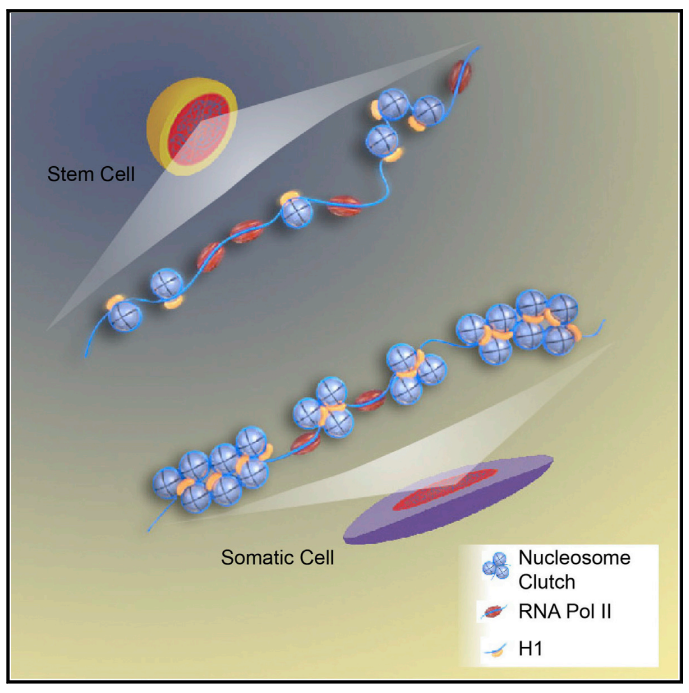
\includegraphics[width=9cm]{Abstract.png}
\end{figure}
\textit{Ricci et al. Chromatin Fibers Are Formed by Heterogeneous Groups of Nucleosomes In Vivo. Cell 2015}
\end{frame}

\begin{frame}{Figure 1. Nucleosomes Are Arranged in Discrete Nanodomains in Interphase Nuclei of Human Somatic Cells}
\begin{figure}
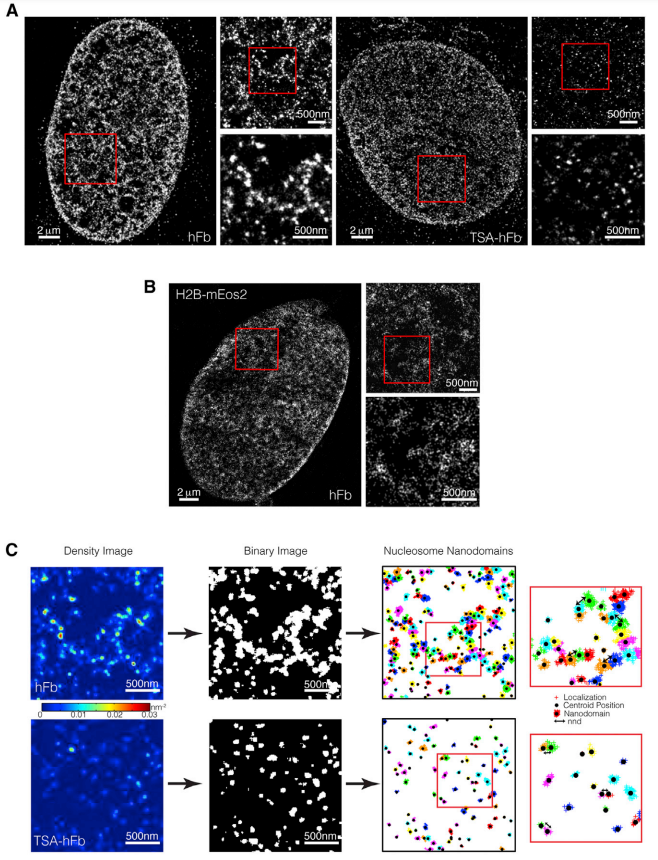
\includegraphics[width=9cm]{Figure-1.png}
\end{figure}
\end{frame}


\begin{frame}{Figure 2. Nucleosomes Are Arranged in Discrete Nanodomains in Interphase Nuclei of Mouse Embryonic Stem Cells}
\begin{figure}
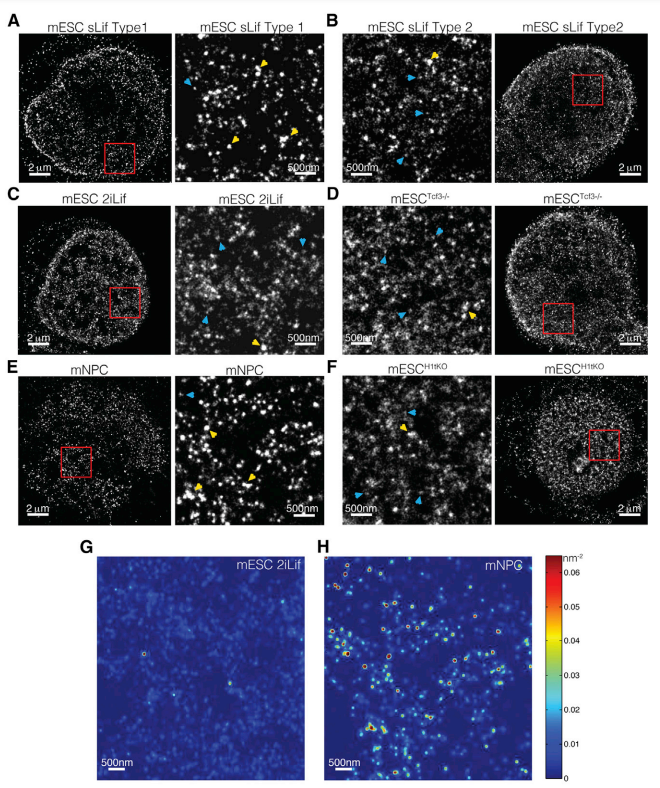
\includegraphics[width=10cm]{Figure-2.png}
\end{figure}
\end{frame}


\begin{frame}{Figure 2. Treatment Conditions}

Transcriptional programs such as cell differentiation are linked to higher order DNA structure. So they manipulate differentiation and analyze structure:

\vspace{0.2in}

Human: 
\begin{itemize}
\item hFb - Human Fibroblast
\item TSA hFB - Human Fibroblast treated with deacetylation inhibitor (decondensation)
\end{itemize}

Mouse:
\begin{itemize}
\item {mESC sLif (maintains ground state but heterogeneous)}
\item {mESC 2iLif (maintains ground state)}
\item {mESC Tcf3 -/- (maintains ground state)}
\item {mESC NPC (differentiated cell)}
\item {mESC H1tKO (KO histone H1 promotes compaction) }
\end{itemize}
\end{frame}

\begin{frame}{Figure 3. The Number of Nucleosomes Inside Clutches Correlates with Cellular State}
\begin{figure}
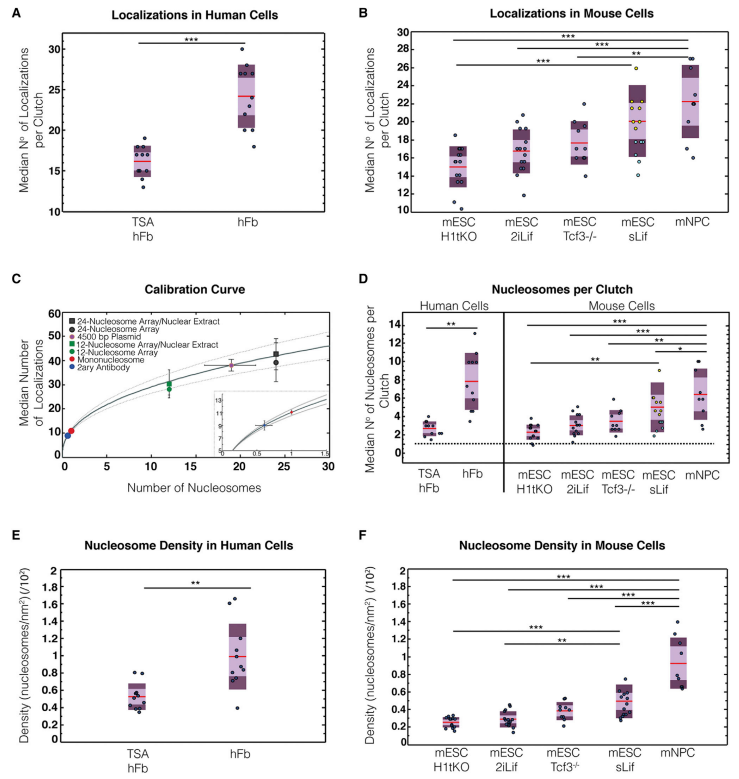
\includegraphics[width=10cm]{Figure-3.png}
\end{figure}
\end{frame}

\begin{frame}{Figure 4. Clutch Size Correlates with Pluripotency Grade in Human-Induced Pluripotent Stem Cells Clones}
**Skip
\begin{figure}
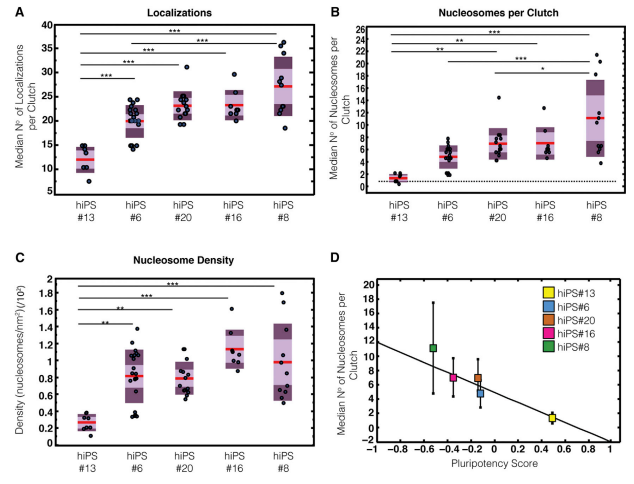
\includegraphics[width=10cm]{Figure-4.png}
\end{figure}
\end{frame}

\begin{frame}{Figure 5. The Linker Histone H1 Increases in Large Clutches and These Correlate with Heterochromatin Markers}
\begin{figure}
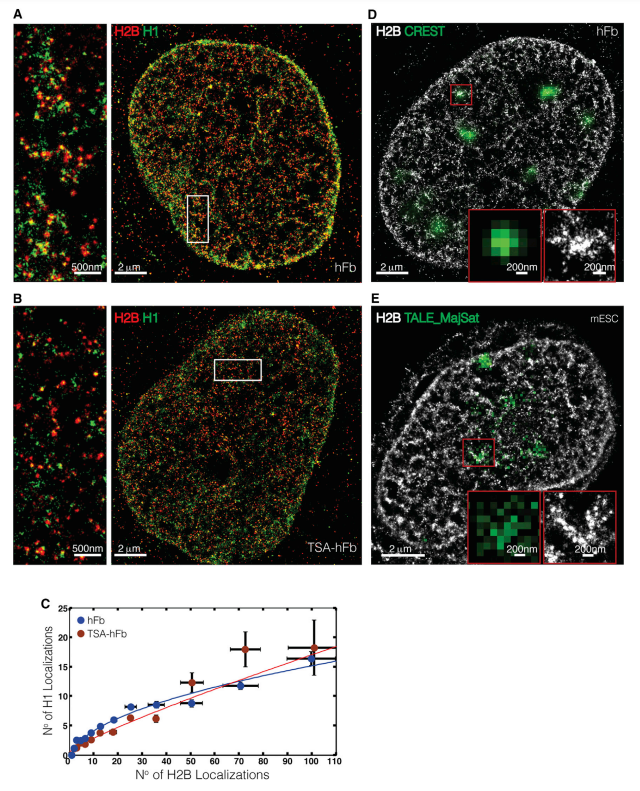
\includegraphics[width=10cm]{Figure-5.png}
\end{figure}
\end{frame}

\begin{frame}{Figure 6. RNA Polymerase II Associates with the Small Clutches}
\begin{figure}
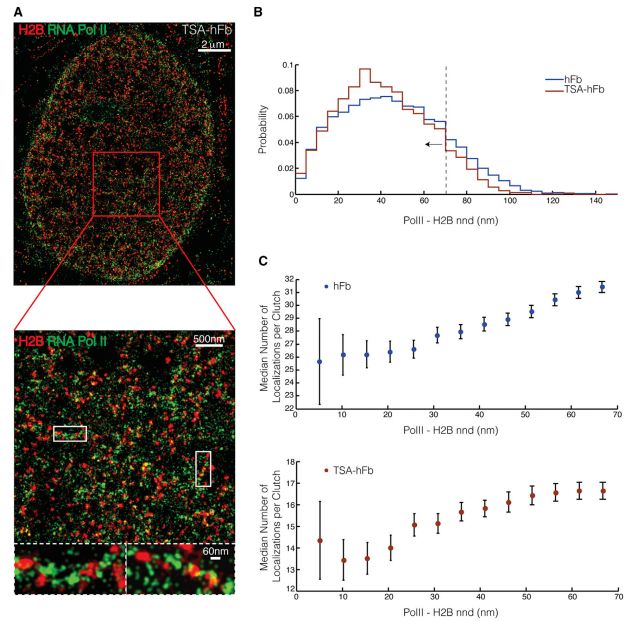
\includegraphics[width=11cm]{Figure-6.png}
\end{figure}
\end{frame}

\begin{frame}{Figure 7. Computer Simulations of Nucleosome Occupancy}
\begin{figure}
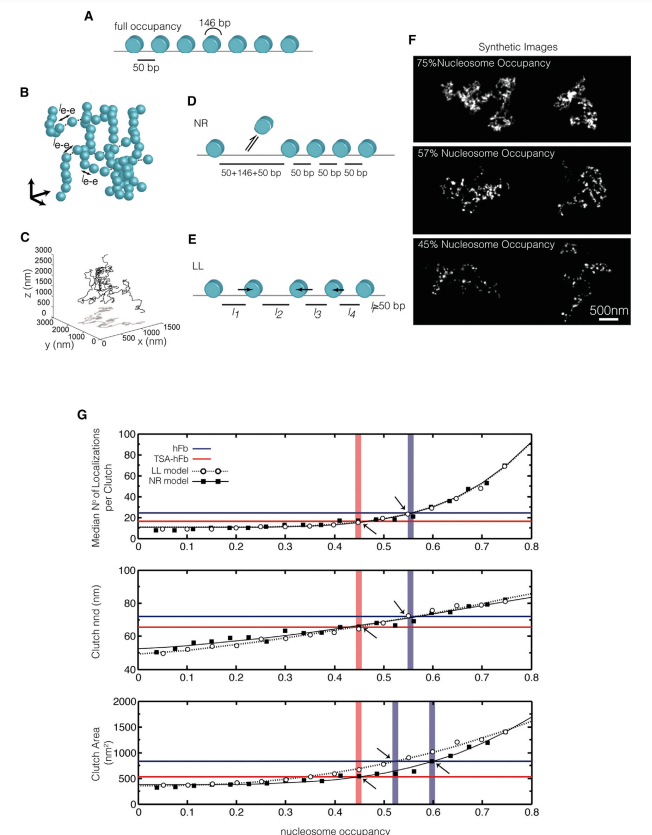
\includegraphics[width=10cm]{Figure-7.png}
\end{figure}
\end{frame}

\end{document}